\section{Complex integration}
Let's first recall from vector analysis: if $\vec{F}: \mathbb{R}^2 \to \mathbb{R}^{2}$ is a vector field such that
\begin{align*} 
	F\left(x_1, x_2\right) = \left(F_1\left(x_1, x_2\right), F_2\left(x_1, x_2\right)\right)
\end{align*}
And $\gamma : \left[a, b\right] \to \mathbb{R}^{2}$ is a $C^{1}$ curve with image $\Gamma$ then:

	\begin{align*} 
		\underbrace{\int_\Gamma Fdl}_{\text{line integral}} &:= \int_a^b F\left(\gamma\left(t\right)\right) \cdot \gamma'\left(t\right)dt
	\end{align*}
	\begin{figure}[h!]
	\centering
	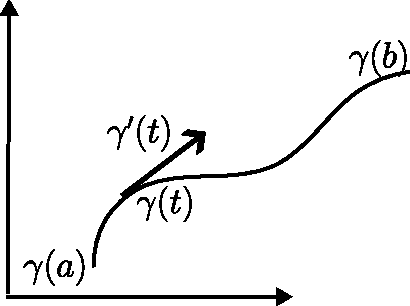
\includegraphics[width=0.3\textwidth]{figure/2026-03-05.pdf}
	\caption{Sorry for the curve}
	\end{figure}
	Here the orientation is \important{important}. We will need to recall some facts:
	\begin{enumerate}
	    \item The line integral is \important{independent} of the parametrisation, but switching orientation creates a negative sign.
		\item If $\gamma: \left[c, d\right] \to \left[a, b\right]$ is one-to-one, out and increasing, then $\gamma$ is a parametrization of $\Gamma$.
		\item If $\gamma$ is closed, meaning $\gamma\left(a\right) = \gamma\left(b\right)$ and curl$F = 0$ ($= \nabla \times F$) in the 'interior' of $\Gamma$, then we have that:
			\begin{align*} 
				\int_\Gamma Fdl = 0
			\end{align*}
			This is a consequence from Stokes theorem
		\item A curve is called:
			\begin{itemize}
				\item \important{simple} if it has no self intersections
				\item \important{regular} if $\gamma' \neq 0$ $ \forall x \in \left[a, b\right]$
			\end{itemize}
	\end{enumerate}
	Now we will define a similar notion of line integrals for complex functions.
	\begin{definition}
		Let $\gamma: \left[a, b\right] \to \mathbb{C}$ be a regular curve that parametrises $\Gamma \subseteq \mathbb{C} $. Let $f : \Gamma \to \mathbb{C}$ be continuous.\\
		$ $\\
		Then we define the line integral of $f$ along $\Gamma$ by:
		\begin{align*} 
			\int_{\Gamma}f\left(z\right)dz =  \int_{\gamma}f\left(z\right)dz := \int_a^b f\left(\gamma\left(t\right)\right) \cdot  \gamma'\left(t\right)dt
		\end{align*}
	\end{definition}
	\begin{framedremark}
	The $\int_\gamma$ is a slight abuse of notation
	\end{framedremark}
	Usually we write $-\Gamma$ to mean the curve $\Gamma$ with the \important{reverse} orientation. In this case we have:
	\begin{align*} 
		\int_{-\Gamma}f\left(z\right)dz = - \int_{\Gamma}f\left(z\right)dz
	\end{align*}

	\begin{framedremark}
	The value of this line integral is independent of the parametrization of $\gamma$ as long as the orientation is preserved.
	\end{framedremark}

	\begin{parag}{Example}
	    Let $\Gamma$ be the unit half circle around $z= 0$, parametrized counter clockwise:
		\begin{center}
		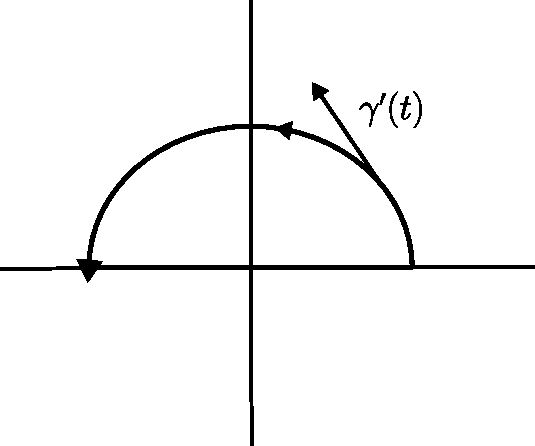
\includegraphics[width=0.35\textwidth]{figure/2026-03-05_1.pdf}
		\end{center}
		\begin{align*} 
			\gamma : [0, \pi] \to \mathbb{C}\\
			\gamma \left(t\right) = e^{it}\\
			\gamma'\left(t\right) = ie^{it}
		\end{align*}
		We seek to integrate $f\left(z\right) = z^2$ over $\Gamma$: 
		\begin{align*} 
			\int_\Gamma z^2dz &= \int_0^\pi \left(e^{it}\right)^2 ie^{it}dt\\
							  &= i \int_0^\pi e^{3it}dt = i \left[\frac{e^{3it}}{ti}\right]_0^\pi =  -\frac{2}{3}
		\end{align*}
\begin{subparag}{Remark}
    Above we used the fundamental theorem of calculus. For more general function, one splits the integrands into real and imaginary part and computes the two real integrals separately.
\end{subparag}
	\end{parag}
	\begin{parag}{Example ii}
	    Let $\Gamma$ be the unit circle oriented counter-clockwise. We will use the same $\gamma$ as before but we will extend its domain of definition:
		\begin{align*} 
			\gamma: [0, 2\pi] \to \mathbb{C}\\
			\gamma\left(t\right) := e^{it}
		\end{align*}
		With again $\gamma'\left(t\right) = ie^{it}$. We try to compute $f\left(z\right)= z^2$:
		\begin{align*} 
			\int_\Gamma z^2dz &=  \int_0^{2\pi}\left(e^{it}\right)^2 ie^{it}dt\\
							  &= \int_0^{2\pi}e^{3it}dt\\
							  &= i \left[\frac{e^{3it}}{3i}\right]_0^{2\pi} = 0
		\end{align*}
		This is a special case of the Cauchy integral theorem (that we will see later).
	\end{parag}
	\begin{parag}{Example iii}
	    Let $\Gamma$ and $\gamma$ be defined as above. We will take this time $f\left(z\right) = \frac{1}{z}$.
		\begin{align*} 
			\int_\Gamma \frac{1}{z}dz &= \int_0^{2\pi}\frac{1}{e^{it}}ie^{it}dt\\
									  &=  \int_0^{2\pi}idt = 2\pi i \neq 0
		\end{align*}
	\end{parag}
	\begin{parag}{Example iv}
		Now let $f\left(z\right) = \frac{1}{z^2}$:
		\begin{align*} 
			\int_\Gamma \frac{1}{z^2} &=  \int_0^{2\pi}\frac{1}{\left(e^{it}\right)^2}ie^{it}dt = i\int_0^{2\pi}e^{-it}dt\\
									  &= -\left[e^{it}\right]_0^{2\pi} = 0
		\end{align*}
	\end{parag}
	
	

	
	
	
\subsection{Cauchy's Theorem}
The Cauchy theorem tells us what the value of a complex integral is on general constraints:
\begin{theoreme}
	Let $U \subseteq \mathbb{C}$ open and simply connected set and let $\Gamma$ be a closed and piecewise regular curve inside $U$. Let $f : U \to \mathbb{C}$ be holomorphic. Then:
	\begin{align*} 
		\int_\Gamma f\left(z\right)dz = 0
	\end{align*}
\end{theoreme}
\begin{parag}{Geometric intuition}
	\begin{definition}
    A domain is said simply connected when it is a domain with only one component and '\textit{no holes}' e.g. $\mathbb{C}, \left\{z \in \mathbb{C}: \left\|<\right\| \leq 1\right\}$, while $\mathbb{C}^{\ast}$ is not simply connected.
	\end{definition}
	\begin{definition}
	\important{Piecewise regular} $\Gamma$ means $\Gamma$ might have finitely many curves, e.g. square
	\end{definition}
	\begin{center}
	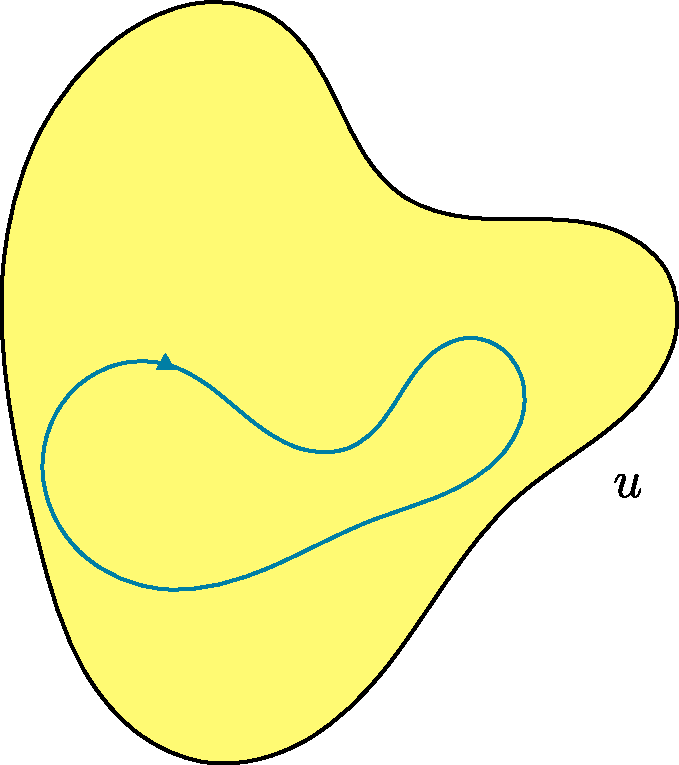
\includegraphics[width=0.3\textwidth]{figure/2026-03-05_2.pdf}
	\end{center}
	
	\begin{subparag}{Why is this true?}
	    Let $\gamma\left(t\right) = \alpha\left(t\right) + \beta\left(t\right)i$ a parametrization $\Gamma_1$ and:
		\begin{align*} 
			f\left(x + yi\right) = u\left(x, y\right) + iv\left(x, y\right)
		\end{align*}
		Then the integral gives us:
		\begin{align*} 
			\int_\Gamma f\left(z\right)dz &= \int_a^b f\left(\gamma\left(t\right)\right) \cdot  \gamma'\left(t\right)dt\\
										  &= \int_a^b \left[u\left(\gamma\left(t\right)\right) + iv\left(\gamma\left(t\right)\right)\right] \cdot \left[\alpha'\left(t\right) + \beta'\left(t\right)i\right] dt\\
										  &= \int_a^b \left[u\left(\gamma\left(t\right)\right)\alpha'\left(t\right) - v\left(\gamma\left(t\right)\right) - \beta'\left(t\right)\right] dt \\
										  &+ i\int_a^b \left[u\left(\gamma\left(t\right)\right)\beta'\left(t\right) + v\left(\gamma\left(t\right)\right)\alpha'\left(t\right)\right]dt\\
										  &=  \int_a^b \begin{pmatrix} u\left(\gamma\left(t\right)\right) \\ -v\left(\gamma\left(t\right)\right) \end{pmatrix}  \cdot \begin{pmatrix} \alpha'\left(t\right) \\ \beta'\left(t\right) \end{pmatrix} dt + i \int_a^b \begin{pmatrix} v\left(\gamma\left(t\right)\right) \\ u\left(\gamma\left(t\right)\right) \end{pmatrix} \cdot \begin{pmatrix} \alpha'\left(t\right) \\ \beta'\left(t\right) \end{pmatrix} dt\\
			&= \int_a^b Fdl + i \int_a^b Gdl
		\end{align*}
		And by Green's theorem we have:
		\begin{align*} 
			= \int_{iut \Gamma} \text{curl}F dxdy + i \int_{iut \Gamma} \text{curl} G dxdy
		\end{align*}
		And if we compute the curl:
		\begin{align*} 
			\text{curl}F &= \frac{\partial F_2}{\partial x_1}  - \frac{\partial F_1}{\partial x_2}  = -\frac{\partial v}{\partial x}  - \frac{\partial u}{\partial y} \\
			\text{curl}F &= \frac{\partial G_2}{\partial x_1}  - \frac{\partial G_1}{\partial x_2}  = \frac{\partial u}{\partial x}  - \frac{\partial v}{\partial y} 
		\end{align*}
		And by the Cauchy Riemann equations both are equal to $0$. Hence: 
		\begin{align*} \int_\Gamma f\left(z\right)dz = 0 \end{align*}
		
	\end{subparag}
	Notice here we used that since $u$ is simply connected and $\Gamma \subseteq u$ we have  int $ \Gamma \subseteq u$, so $F, G$ are defined on int $ \Gamma$
\end{parag}


\begin{parag}{Example}
	Let $\Gamma$ be the unit circle, $f\left(z\right) = z^2$. By applying Cauchy theorem to $u = \mathbb{C}$, then:
	\begin{align*} 
		\int_\Gamma f\left(z\right)dz = 0
	\end{align*}
\end{parag}
\begin{parag}{Example ii}
    Again, let's take $\Gamma$ to be the unit circle and $f\left(z\right) = \frac{1}{z}$.\\
	$ $\\
	We are looking for a simply connected domain which contains the unit circle \important{and} $f$ is holomorphic. But this is not possible because $f$ is only holomorphic on $\mathbb{C}^{\ast}$ and there is no simply connected domain $U \subseteq \mathbb{C}^{\ast}$ that contains $\Gamma$. Therefore, Cauchy's theorem does not apply. (indeed, as we have calculated above, $\int_\Gamma f\left(z\right)dz \neq 0$)
\end{parag}


\begin{parag}{Example iii}
    Let $f\left(z\right) = \frac{1}{z}$, $\Gamma =  \left\{z \in \mathbb{C}: \left\|z - 2\right\|= 1\right\}$.\\
	$ $\\
	For instance let us take the domain $u =  \left\{ \text{Re} > 0\right\}$ which is a simply connected domain which contains $\Gamma$, and where $f$ is holomorphic on $u$. By the Cauchy theorem, we have that:
	\begin{align*} 
		\int_\Gamma f\left(z\right)dz = 0
	\end{align*}
\end{parag}
In practice, we'll apply Cauchy's theorem as follows:
\begin{itemize}
	\item Given $\Gamma$ and $f$
	\item Find a simply connected open domain $U \subseteq \mathbb{C}$ such that:
		\begin{itemize}
			\item $U$ contains $\Gamma$ and
			\item $f$ is holomorphic on $U$
		\end{itemize}
\end{itemize}

There is an extension of Cauchy's theorem which is nice for application:
\begin{theoreme}
Let $\Gamma_0, \Gamma_1$ be closed and simple regular curves such that $\Gamma_1 \subseteq $ int $\Gamma_0$. Let $\gamma_0, \gamma_1$  be parametrization of $\Gamma_0, \Gamma_1$ with the same orientation.\\
$ $\\
If $f$ is holomorphic on our two curves, then:
\begin{align*} 
	\int_{\Gamma_0}f\left(z\right)dz = \int_{\Gamma_1} f\left(z\right)dz
\end{align*}
\end{theoreme}
\begin{center}
    

	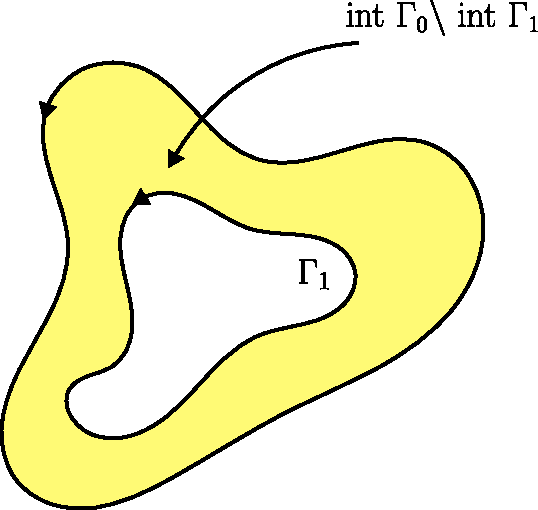
\includegraphics[width=0.3\textwidth]{figure/2026-03-05_3.pdf}
\end{center}
This allows us to compute complicated line integral by an easy line integral. 

\begin{parag}{How to shows this?}
    Since $f$ is holomorphic on int $\sigma$ and  int$\sigma_2$, by Cauchy's theorem:
	\begin{align*} 
		\int_{\sigma_1}f\left(z\right)dz = 0 = \int_{\sigma_0} f\left(z\right)dz
	\end{align*}
	So we have that:
	\begin{align*} 
		0 &= \int_{\sigma_0}f\left(z\right)dz + \int_{\sigma_1}f\left(z\right)dz\\
		&= \int_{\gamma_0}f\left(z\right)dz - \int_{\gamma_1}f\left(z\right)dz  + 0
	\end{align*}
\end{parag}
\subsubsection{Cauchy integral formula}
\begin{theoreme}
Suppose $D \subseteq \mathbb{C}$ is open and $f : D \to \mathbb{C}$ is holomorphic.\\
$ $\\
If $z_0 \in D$,
\begin{align*} 
	f\left(z_0\right) =  \frac{1}{2\pi i}\int_{\gamma}\frac{f\left(z\right)}{z - z_0}dz
\end{align*}
For every closed, simple curve $\gamma$ inside $D$ whose interior contains $z_0$ and is counter-clockwise oriented.
\end{theoreme}
\begin{parag}{How to show this?}
    First:
	\begin{align*} 
		\frac{f\left(z\right)}{z - z_0}
	\end{align*}
	is holomorphic on $D \setminus \left\{z_0\right\}$. By extended Cauchy's theorem we have:
	\begin{align*} 
		\int_\gamma \frac{f\left(z\right)}{z - z_0} =  \int_{\gamma_1} \frac{f\left(z\right)}{z - z_0}dz
	\end{align*}
	where $\gamma_1 : \left[0, 2\pi\right] \to \mathbb{C}$, $\gamma_1\left(t\right) =  z_0 + re^{it}$, for a small $r$. Hence:
	\begin{align*} 
		\int_\gamma \frac{f\left(z\right)}{z - z_0} dz &=  \int_{\gamma_1}\frac{f\left(z\right)}{z - z_0}dz\\
		&= \int_0^{2\pi}\frac{f\left(z_0 + re^{it}\right)}{re^{it}}ire^{it}dt\\
		&= i \int_0^{2\pi} f\left(z_0 + re^{it}\right) dt \to i2\pi f\left(z_0\right) \text{ as }  r \to 0
	\end{align*}
	using that $f$ is continuous at $z_0$.
\end{parag}



